\subsection{Accuracy (P-R) and Overlap (vs. SP)}
We run our action conceptualization algorithms on the two dataset,
and report a snapshot of top 5 subject and object concepts extracted
by local search from the web sentence data
for each verb in Verb-20 in \tabref{tab:top5result}.
To quantitatively evaluate the resulting action concepts,
we design three metrics to evaluate our action concept lexicon.
Since we mainly focus on evaluating the object concepts extracted by
our approaches, we abuse using the term \emph{argument}
to refer to object of the verbs in the following experiments.

\begin{table*}[th]
\centering
\caption{Top 5 Subject and Object Concepts Extracted by Local Search on Web Sentence Data}
\small
% Table generated by Excel2LaTeX from sheet 'Sheet1'
\begin{tabular}{|l|l|l|}
    \hline
    Verbs & Subject & Object \\
    \hline \hline
    bring & person, event, service, company, group & issue, person, food, gift, group \\
    \hline
    carry & person, word, store, vehicle, group & information, person, food, weapon, supply \\
    \hline
    connect & device, person, word, project, site & device, person, attribute, unit, group \\
    \hline
    cut   & person, company, part, group, time & material, cost, tool, life, time \\
    \hline
    define & document, parameter, section, object, user & term, parameter, function, purpose, method \\
    \hline
    eat   & person, animal, word, group, food & food, word, time, cost, plant \\
    \hline
    help  & information, program, tool, food, organization & person, group, matter, symptom, business \\
    \hline
    hit   & word, player, vehicle, part, company & person, market, button, target, surface \\
    \hline
    keep  & person, word, part, company, food & information, person, part, food, animal \\
    \hline
    operate & service, company, person, device, factor & business, facility, system, vehicle, program \\
    \hline
    perform & person, service, group, artist, company & task, procedure, work, process, test \\
    \hline
    play  & person, factor, player, band, game & game, factor, role, character, part \\
    \hline
    read  & person, information, group, book, software & information, book, work, article, skill \\
    \hline
    release & company, band, medium, datum, role & information, name, game, film, work \\
    \hline
    report & person, company, datum, group, medium & information, symptom, purpose, incident, crime \\
    \hline
    select & user, key, tab, list, committee & item, topic, parameter, role, group \\
    \hline
    spend & person, group, company, time, department & time, life, money, game, point \\
    \hline
    submit & person, information, group, company, department & information, application, material, case, name \\
    \hline
    visit & person, information, group, program, team & facility, section, country, school, website, page \\
    \hline
    wear  & person, part, information, model, class & clothing, jewelry, stuff, color, shoe \\
    \hline
    \end{tabular}%
\label{tab:top5result}
\end{table*}


\subsubsection{Accuracy}
We use precision, recall and $F_1$ measure to evaluate the accuracy of our
approaches.

\textbf{Precision}: We use precision to evaluate the quality of concepts produced by each
algorithm. For a given verb, a good concept for argument is not only required to
cover more arguments in the dataset, but also contain less entities
that cannot be the argument for that verb. For each algorithm,
we build a ground truth dataset from Verb-20 by
sampling 10 entities for each top-10 argument concept discovered by the algorithm.
To make more typical entities to be more easily sampled out,
the sampling is conducted according to the typicality of the entities.
The resulting annotation set comprises 2,000 unique entities.
Each entity is then labeled whether it is a correct argument to the corresponding verb
 by 3 human judges. The definition of precision score for each verb is showed below.
$$
Precision = \frac{\sum_{c \in C}|E_c|\times Precision(c)}{\sum_{c \in C}{|E_c|}}
$$
$$
Precision(c)=\frac{\#\ \mbox{of\ correct\ arguments\ belongs\ to}\ c}{10}
$$
, where $|E_c|$ is the number of entities in concept $c$ and
$C$ is the set of top 10 argument concepts discovered by the algorithms.

We compare the proposed two algorithms, i.e., greedy solution(GS)
and local search(LS) to selectional preference(SP) in the sense
of precision on web sentence data, as well as local search on
Google syntactic N-gram data. The overall precision of the 20 verbs
is reported in \figref{fig:precision}.
For all the algorithms, we keep the top-k concepts for the argument of
each verb. As the number of concepts grows, the precision decrease
among all the approaches. The greedy solution loses in terms of precision
comparing to local search and selectional preference because it prefers
to select general concepts to minimize the number of concepts.
Simulated annealing is able to jump out of the local optimal and 
find a solution that close to the global optimal.  
The comparison among the three approaches on web sentence dataset
shows that our local search algorithm is enable to find concepts
with proper granularity, i.e., covering most correct arguments but
less incorrect arguments. We also compare the precision of
applying local search to web sentence data with that to Google
syntactic N-grams.

%% Table generated by Excel2LaTeX from sheet 'precision'
%\begin{table}[th]
%\centering
%\caption{Precision}
%\small
%\begin{tabular}{|l|ccc|l|ccc|}
%\hline
%      Verb &         LS &         SP &       GS &       Verb &         LS &         SP &       GS \\
%\hline \hline
%     bring &      0.97  &      0.89  &      0.93  &    perform &      0.62  &      0.65  &      0.60  \\
%\hline
%     carry &      0.96  &      0.97  &      0.80  &       play &      0.72  &      0.70  &      0.68  \\
%\hline
%   connect &      0.89  &      0.78  &      0.42  &       read &      0.62  &      0.65  &      0.64  \\
%\hline
%       cut &      0.83  &      0.88  &      0.90  &    release &      0.86  &      0.75  &      0.88  \\
%\hline
%    define &      0.95  &      0.95  &      0.93  &     report &      0.94  &      0.99  &      0.86  \\
%\hline
%       eat &      0.56  &      0.57  &      0.34  &     select &      0.96  &      0.92  &      0.95  \\
%\hline
%      help &      0.81  &      0.91  &      0.80  &      spend &      0.49  &      0.81  &      0.68  \\
%\hline
%       hit &      0.84  &      0.57  &      0.68  &     submit &      0.91  &      1.00  &      0.97  \\
%\hline
%      keep &      0.88  &      0.95  &      0.91  &      visit &      0.77  &      0.39  &      0.67  \\
%\hline
%   operate &      0.79  &      0.82  &      0.86  &       wear &      0.54  &      0.71  &      0.26  \\
%\hline
%\end{tabular}
%\label{tab:precision}
%\end{table}

%\begin{table}[th]
%\centering
%\caption{Precision}
%\small
%% Table generated by Excel2LaTeX from sheet 'Sheet1'
%\begin{tabular}{|l|ccc|l|ccc|}
%\hline
%      Verb &         SP &         GS &         LS &       Verb &         SP &         GS &         LS \\
%\hline \hline
%     bring &      0.91  &      0.91  &      0.95  &    perform &      0.61  &      0.48  &      0.66  \\
%\hline
%     carry &      0.97  &      0.87  &      0.94  &       play &      0.54  &      0.58  &      0.54  \\
%\hline
%   connect &      0.84  &      0.75  &      0.89  &       read &      0.58  &      0.31  &      0.66  \\
%\hline
%       cut &      0.57  &      0.75  &      0.47  &    release &      0.63  &      0.55  &      0.80  \\
%\hline
%    define &      0.95  &      1.00  &      0.95  &     report &      0.97  &      0.89  &      0.95  \\
%\hline
%       eat &      0.50  &      0.34  &      0.46  &     select &      0.96  &      1.00  &      0.95  \\
%\hline
%      help &      0.94  &      0.55  &      0.82  &      spend &      0.61  &      0.31  &      0.17  \\
%\hline
%       hit &      0.70  &      0.95  &      0.89  &     submit &      0.90  &      0.82  &      0.80  \\
%\hline
%      keep &      0.82  &      0.87  &      0.86  &      visit &      0.36  &      0.57  &      0.80  \\
%\hline
%   operate &      0.74  &      0.23  &      0.80  &       wear &      0.26  &      0.23  &      0.43  \\
%\hline
%\end{tabular}
%\label{tab:precision}
%\end{table}

\textbf{Recall}: Recall is used to evaluate the coverage on correct
objects of concepts produced by each algorithm.
We create two gold standard datasets to evaluate
the recall of action concepts extracted from the
two datasets, i.e., web sentences and Google syntactic
N-gram. On one hand, we manually label 100 correct arguments for each
verb in Verb-20 from the Google syntactic N-gram data
to evaluate the recall of action concepts extracted
from web sentences. On the other hand, we use a
manually annotated set of 100 correct arguments for
each verb in Verb-20 from web sentences to compute
the recall of action concepts extracted from Google
syntactic N-gram. The 100 correct arguments for
each verb are collected randomly and evaluated
by three human judges. With the ground truth, we check
if those correct arguments are covered by one of the concepts
extracted for each algorithm. The definition of recall for each verb
is showed below.
$$
Recall=\frac{\sum_{a \in A}{I(a,C)}}{|A|}
$$
, where $A$ is the set of arguments in the web/Google dataset
for the verb; Function $I(a,C)$ is defined as:
$$
I(a,C)=
\begin{cases}
1 & if\ \exists c \in C\ and\ a\ IsA\ c\\
0 & otherwise
\end{cases}
$$

We report the recall of our approaches as well as
selectional preference in \figref{fig:recall}.
Greedy solution achieves a very high recall, because
it prefers larger concepts. Local search and selectional
preference performs similar in terms of recall.

\textbf{$F_1$ measure}: We examine the $F_1$ measure to
incorporate the precision and recall for a overall
evaluation of accuracy of the algorithms. $F_1$ is
define as follows:
$$
F_1=\frac{2\cdot Precision \cdot Recall}{Precision + Recall}
$$
The $F_1$ measure of all the algorithms are summarized in
\figref{fig:f1}. Greedy solution is fast and achieves good accuracy
in the top three concepts, while appears to be less efficient
when the number of concepts become large.
Local search outperforms
selectional preference in all settings. In the comparison
of the two datasets, action concepts extracted from web sentence
data are more accurate than those from Google syntactic N-grams.
The reason is our web sentence data contains more action
instances for each verb which produces a large mount of evidence
to support our algorithm.

\begin{figure*}[th]
\begin{minipage}[t]{0.66\columnwidth}
\centering
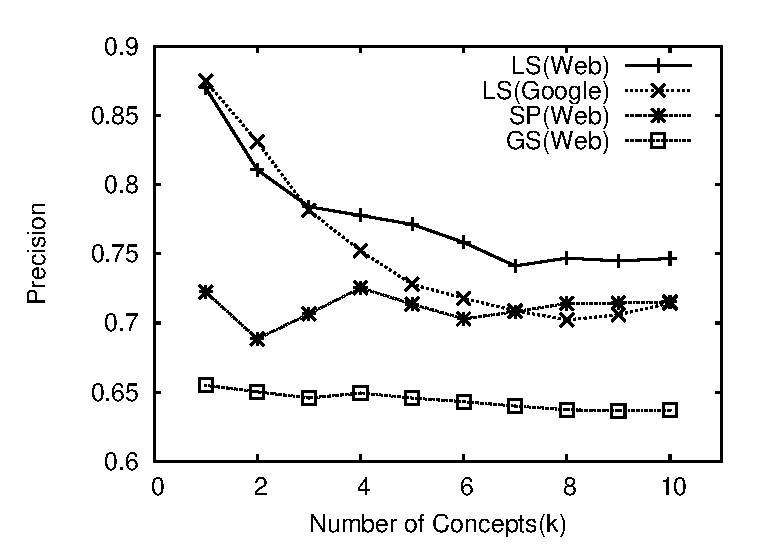
\epsfig{file=figure/precision.eps,width=\columnwidth}
\caption{Precision}
\label{fig:precision}
\end{minipage}
\begin{minipage}[t]{0.66\columnwidth}
\centering
\epsfig{file=figure/recall_new.eps,width=\columnwidth}
\caption{Recall}
\label{fig:recall}
\end{minipage}
\begin{minipage}[t]{0.66\columnwidth}
\centering
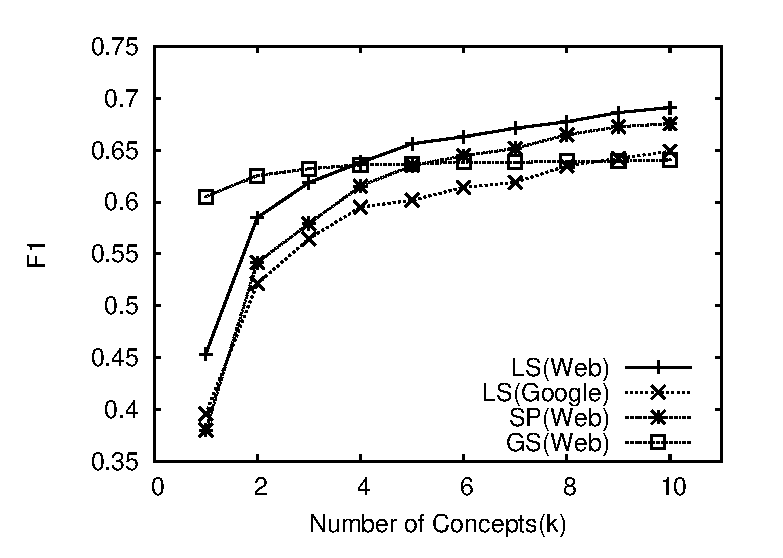
\epsfig{file=figure/f.eps,width=\columnwidth}
\caption{$F_1$ Measure}
\label{fig:f1}
\end{minipage}
\end{figure*}

%\begin{table}[th]
%\centering
%\caption{Recall}
%\small
%% Table generated by Excel2LaTeX from sheet 'Sheet1'
%\begin{tabular}{|l|ccc|l|ccc|}
%\hline
%      Verb &         SP &         GS &         LS &       Verb &         SP &         GS &         LS \\
%\hline
%     bring &      0.85  &      0.88  &      0.83  &    perform &      0.85  &      0.78  &      0.70  \\
%\hline
%     carry &      0.76  &      0.87  &      0.72  &       play &      0.63  &      0.83  &      0.80  \\
%\hline
%   connect &      0.59  &      0.67  &      0.67  &       read &      0.64  &      0.83  &      0.72  \\
%\hline
%       cut &      0.76  &      0.90  &      0.67  &    release &      0.75  &      0.73  &      0.46  \\
%\hline
%    define &      0.71  &      0.74  &      0.72  &     report &      0.73  &      0.84  &      0.69  \\
%\hline
%       eat &      0.78  &      0.82  &      0.87  &     select &      0.73  &      0.78  &      0.69  \\
%\hline
%      help &      0.75  &      0.71  &      0.75  &      spend &      0.62  &      0.74  &      0.74  \\
%\hline
%       hit &      0.58  &      0.81  &      0.66  &     submit &      0.66  &      0.73  &      0.70  \\
%\hline
%      keep &      0.72  &      0.81  &      0.85  &      visit &      0.59  &      0.82  &      0.48  \\
%\hline
%   operate &      0.83  &      0.75  &      0.87  &       wear &      0.79  &      0.89  &      0.83  \\
%\hline
%\end{tabular}
%\label{tab:recall}
%\end{table}

\subsubsection{Overlap}
Ideally the intersection between every two concepts in the result
should be as small as possible, which means each concept should
correspond to a distinct meaning.
We define an overlap score simply as:
\[
Overlap = \frac{2\cdot\sum_{c_1,c_2\in C}{\frac{|E_{c_1} \cap E_{c_2}|}{min\{|E_{c_1}|,|E_{c_2}|\}}}}{|C|(|C|-1)},
\]
where $C$ is the set of top 10 argument concepts discovered by the algorithms;
variables $E_{c_1}$ and $E_{c_2}$ are the entity sets of $c_1$ and $c_2$, respectively.
The intuition is that, if there is no overlap between every two concepts, each argument
will be covered by only one concept, then overlap score will be 0 which is the best.
The more overlap, the more concepts one object being covered, so that the overlap score
will be high. The overlap score of action concepts extracted by the three algorithms
as reported in \tabref{tab:overlap}. Most of the verbs do not overlap in greedy solution,
because when we pick a concept we choose from concepts that do not violate the overlap
constrain. Overlap of local search is slightly higher than GS, but it still guarantees
the overlap constrain. In contrast, selectional preference tends to generate general
concepts which results in a high overlap score.

\begin{table}[th]
\small
\centering
\caption{Overlap}
\begin{tabular}{|r|c|c|c||r|c|c|c|}
\hline
Verbs&	LS&	GS&	SP&    Verbs&	LS&	GS&	SP	\\ \hline\hline
eat	&0.02	&0.01	&0.15 & report	&0.02	&0.01	&0.16 \\ \hline
perform	&0.03	&0.01	&0.15 & select	&0.03	&0.01	&0.12\\ \hline
play	&0.02	&0.01	&0.10 & operate	&0.03	&0.00	&0.12\\ \hline
submit	&0.04	&0.01	&0.16 & bring	&0.02	&0.01	&0.22\\ \hline
wear	&0.03	&0.01	&0.29 & visit	&0.02	&0.01	&0.05\\ \hline
release	&0.02	&0.01	&0.04 & hit	&0.03	&0.01	&0.17\\ \hline
define	&0.03	&0.00	&0.20 & help	&0.04	&0.01	&0.14\\ \hline
keep	&0.03	&0.01	&0.12 & spend	&0.03	&0.01	&0.34\\ \hline
carry	&0.03	&0.01	&0.23 & read	&0.02	&0.01	&0.10\\ \hline
cut	&0.03	&0.01	&0.12 & connect	&0.03	&0.01	&0.10\\ \hline
\end{tabular}
\label{tab:overlap}
\end{table}


